\part{Les Mondes Fédéraux}

\begin{center}
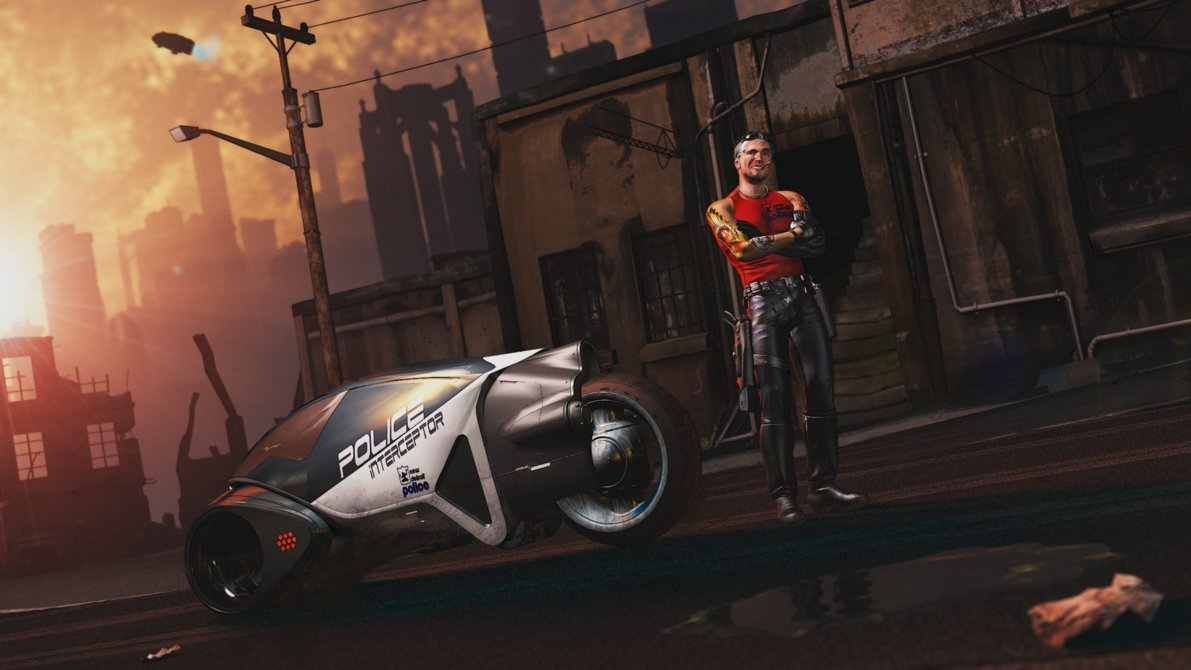
\includegraphics[scale=0.38]{Img/sunset}
\end{center}

\chapter{Vivre dans les mondes Fédéraux}

\begin{multicols}{2}

\section{Monnaie}

Une des premières décisions prisent par la seconde fédération a été de créer une monnaie commune : le crédit fédéral. Elle est devenue très vite la monnaie de référence et d'échange interplanétaire. Malgré la guerre, elle est toujours utilisée et reconnue partout. Toutefois, chaque nation à conservé sa propre monnaie et continue à l'utiliser pour les transactions internes. 

Deux moyens de paiement sont en général utiliser :
\begin{itemize}
\item \textbf{La sphère} est le moyen de paiement pour les achats de la vie courante. Les principales données du compte en banque sont liés au pad de l'utilisateur. Au moment du paiement, celui-ci est directement transmis à l'organisme banquier en utilisant les bulles de réseaux. Le paiement est automatiquement validé. Il n'y a aucune validation de la solvabilité interstellaire de celui qui effectue l'achat. Un état du compte en banque est donc tenu localement avec une autorisation de découvert. Le montant de l'autorisation est réactualisé en fonction des informations transmises par l'organisme banquier.
\item Lorsqu'il s'agit de grosses sommes, il est de coutume d'utiliser \textbf{un disques} de paiement. Ce sont sont des composants certifiés par un organisme banquier qui contiennent virtuellement de l'argent. Ils sont très pratique pour emmener de l'argent avec soit durant un voyage interstellaire. Les petits commerçants ne sont toutefois pas équipé pour débiter de l'argents dessus, il est donc conseillé de transferé de l'argent vers son compte local lors de l'arrivée sur une nouvelle planète.

\end{itemize}

\section{Communication}

Les planètes fédérales sont équipés de systèmes de rélais par satellite ou balise au sol qui permettent une communication instantannée sur sa surface. Pour envoyer un message sur une autre planète du système, on utilise en général un laser qui permet une latence réduit à seulement quelques minutes. 

Pour l'instant, aucune solution technique n'existe pour l'interstellaire. La corporation malTech a mis en place une infrastructure postale. Dans chaque système, une balise permet le dépôt et la récupération des messages interstellaires. Des vaisseaux postaux viennent faire l'échange avant de partir vers un autre système solaire. En plus des vaisseaux postaux, malTech paye de nombreux capitaines de vaisseaux civiles en leur demandant d'effectuer le transfert durant leurs propres voyages. En général, un message peut donc trouver sa cible en moins d'un mois même quand elle se trouve à l'autre bout des mondes fédéraux.

\section{Domaines technologiques}

\subsection{Génétique et Biotech}

La génétique et la biotech sont deux domaines directement liés qui ouvre des milliards de perspectives… Clonage, amélioration génétique, ou même la recherche de l’immortalité… Chacune des races de la fédération a un point commun avec les autres: l’ADN. Bien sûr, la structure même de l’ADN présente des variations. Les Snagirs par exemple possèdent un ADN à 5 branches formant une sorte d’étoile. 

Toutefois, la génétique est un sujet de débat très important dans la fédération galactique. En effet la génétique est une science qui peut s’avérer dangereuse. La génétique permet en effet la conception d’armes mortelles sélectives, qui permettraient d’effectuer un génocide sans aucun risque pour les autres races. 

De plus la génétique ouvre le champ à la folie des plus grands mégalomanes : l’immortalité.

Après un très long débat, le Sénat a donc décidé de fixer des règles très précises empêchant le développement de technologie génétique trop perfectionnée. Il a été décidé de cantonner la génétique dans un but strictement médical. De plus, la loi donne à la fédération le droit de contrôler sur l’intégralité des mondes connus, y compris sur les territoires natifs des différentes races.

\subsection{Nanotech}

La nanotechnologie est une science qui semblait très prometteuse pour l’humanité, elle promettait des milliards d’applications autant sur le plan médical que militaire. Toutefois la nanotechnologie possède un désavantage fatal. Les nanorobots sont des structures tellement petites qu’il est impossible de leur appliquer le moindre blindage ce qui a pour conséquence de les rendre hypersensibles.

Par conséquent, la moindre radiation ou même des écarts de gravité trop importants amènent la destruction des nanorobots. Tout passage dans l’espace amène le même problème.

La Nanotech est finalement une science peu rentable, donc abandonnée.

\subsection{Cybernétique}


Il y a 3 types d’implants :
\begin{itemize}
	\item les implants médicaux
	\item les implants utilitaires
	\item les implants militaires
\end{itemize}

Alors que les deux premières catégories sont légales, la dernière catégorie est restreinte à des forces considérées comme militaires (avec la licence adéquate). Toutefois cette interdiction s’arrête aux frontières de l’espace fédéral, les systèmes natifs ont leur propre législation les concernant. La loi sur ce sujet est donc laxiste dans son application.

Les implants médicaux permettent de remplacer un membre perdu ou de compenser la faiblesse d’un ou plusieurs organes.

\parpic[l]{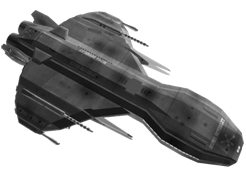
\includegraphics[width=120pt]{image/vaisseau3.png}}Les implants utilitaires sont ceux qui permettent d’améliorer les capacités d’une personne dans une faible mesure : appareil auditif comprenant des amplificateurs, œil cybernétique permettant d’effectuer des zooms, bras permettant d’obtenir une force de levage plus importants.

Les implants militaires sont soit des armes, soit des implants utilitaires possédant des capacités d’amélioration jugées trop importante. Il est parfois difficile de faire la distinction entre un implant militaire et un implant utilitaire.

\end{multicols}

\regle{Comment gerer les implants ?}{
Il existe deux façon de gérer les implants dans Fusina : 
\begin{itemize}
	\item les traits
	\item l'équipement
\end{itemize}
Laquelle utiliser ?

En fait, les deux solutions sont bonnes et utilisables. Le choix se fait en fonction des cas et en accord entre le MJ et les joueurs. Globalement, voici les préconisations que je peux donner :
\begin{itemize}
	\item si l'implant améliore les capacités du personnages dans son ensemble, il faut le décrire via un trait. C'est le cas, par exemple, de réflexes améliorés, d'une armure subdermale, d'un oeil cybernétique, ... Si l'implant fait réellement partie du personnage, on tombe dans cette catégorie  
	\item si l'implant est un ajout qui donne quelques capacités supplémentairse mais ne change pas radicalement le personnage, il peut être considéré comme un équipement. C'est, par exemple, le cas d'une arme greffée sur le bras du personnage.
\end{itemize}
}

\begin{multicols}{2}

\subsection{Intelligences Artificielles}

Avant de parler de l’intelligence artificielle il faut tout d’abord définir correctement ce terme. Peut-être appelé intelligence artificielle tout programme répondant à ces conditions :
\begin{itemize}
	\item Répond à un cycle de décision complexe capable de prendre en compte des éléments imprévu
	\item Possède une capacité d’apprentissage
	\item Peut fonctionner de façon autonome.
\end{itemize}

Couramment les intelligences artificielles sont classées en trois catégories :
\begin{itemize}
	\item Intelligence non-autonome : Il s’agit de l’IA de base qui est capable d’apprendre et d’avoir un comportement sensé. Elle est toutefois incapable d’avoir le sens de l’initiative, des émotions ou de la créativité. Ce type d’IA n’a pas conscience d'elle-même.
	\item Intelligence semi-autonome : Il s’agit de l’IA courante. Elle possède un certain sens de l’initiative et est capable de prendre des décisions d’elle-même en faisant preuve de créativité. Toutefois elle ne ressent pas d’émotions et n’a pas conscience d’elle-même.
	\item Intelligence autonome : Cette catégorie couvre ce que certaine nomment IA véritables. Il s’agit d’IA possédant une réelle conscience d’elles-même. Elles peuvent prendre des décisions en toute autonomie et sont capables d’assimiler des émotions. Finalement ce type d’IA atteint un niveau presque humain.
\end{itemize}

Actuellement les intelligences autonomes et semi-autonomes sont parfaitement légales. Toutefois les IA semi-autonomes ont été sévèrement réglementées pour éviter tout débordement. Les IA autonomes ont par contre été totalement interdites à la demande des Snagirs. 

Dans le passé les Snagirs avait construit de grandes villes gérées automatiquement par des IA autonomes. L’expérience a très mal tourné et a provoqé un grand nombre de mort. Depuis les villes en question ont totalement été abandonnées et vivent encore, en autonomie, tout au fond du grand océan de la planète mère Snagir.

\subsection{Energétique}

Le domaine énergétique est très varié et dépend beaucoup de l’environnement de la planète, station, … Tout d’abord il y a les technologies profitant de l’environnement même, qui sont par nature peu coûteuses mais moins fiables et plus encombrantes. Ces technologies sont :

\begin{itemize}
	\item Le triplet environnement Thermique, Hydraulique, Eolienne
	\item L’énergie solaire
	\item L’énergie profitant des radiations émises par un astre ou un phénomène spatial
\end{itemize}

Ensuite nous pouvons trouver les centrales à fusion et à fission. Ces centrales sont utilisées lorsque le besoin se fait sentir d’avoir une énergie produite en très grande quantité. Ce sont les centrales les plus puissantes mais également les plus coûteuses. 

Concernant l’énergie transportable, la fédération connaît, grâce aux Snagir, un nouveau procédé se basant sur l’utilisation de petites Cristaux de couleurs Rouges : le Sagium. Ces petits cristaux ont des propriétés très intéressantes et étonnantes. Le cristal permet, par un procédé proche de la fusion, de stocker un très grand nombre d’atomes. Le plus étonnant dans les propriétés de ce cristal est qu’il permet une fusion à outrance : les atomes fusionnés deviennent des atomes sur lesquels ont peut employer la fission nucléaire ! 

Les cristaux sont donc utilisés comme des piles pour des micro-générateurs à fission nucléaire. Une grande partie des moteurs de vaisseaux spatiaux utilise ce procédé. L’éjection des atomes crées via la fission permet de propulser le vaisseau à très grande vitesse. L’accélération obtenue est très rapide. La Sagium reste un produit relativement rare et donc très couteux.

Il est à noter que les Teldrims ont également découvert une technique permettant d’utiliser un être vivant comme « pile électrique ». Cette technique est de plus en plus souvent utilisée pour les appareils personnels nécessitant une faible dose d’énergie pour fonctionner.

\subsection{Ressources alimentaires}

Le domaine alimentaire n’a que peu évolué. La principale source reste, et restera probablement toujours, l’agriculture et l’élevage. Bien sûr les techniques ont quand même été bien améliorées. Tout d’abord les cultures sont de plus en plus productives. Elles sont également de plus en plus variées grâce à l’hydroponie ou à la reproduction « sous-dôme » d’un environnement adéquat.

Les méthodes de stockage ont également bien évoluées, on citera notamment la technique de lyophilisation ainsi que les nouvelles méthodes de « compression » des aliments. Seule l’eau reste encore réellement difficile à transporter et demande, pour les vaisseaux et les stations spatiales, un ravitaillement fréquent.  

Dans l’espace, l’eau est une denrée rare et son utilisation est sérieusement contrôlée. 

\subsection{Informatique}

L’informatique est une science qui est devenue tellement courante pour les habitants des fédérations qu’ils en oublient presque son existence. Il n’existe quasiment plus de réseau informatique câblé, tout est maintenant structuré en réseau superposé.

Le réseau le plus vaste est à l’échelle d’un système solaire. Ce réseau sert principalement pour les médias et les télécommunications entre deux planètes. A cause de son échelle importante, ce réseau possède un temps de latence assez énorme (qui peut aller jusqu’à plusieurs minutes). Toute autre action effectuée sur ce réseau demande des habilitations et du matériel spécifique.

Ensuite, nous avons un réseau à l’échelle planétaire. Ce réseau a une fonction similaire à celui d’un système solaire mais possède un temps de latence bien plus acceptable (quelques secondes). Ce réseau possède également une base de données référençant, par exemple, les lois en vigueur sur la planète et les annonces du gouvernement. 

Ensuite, nous avons des réseaux de proximité (aussi appelé réseaux locaux).  Ces réseaux sont ceux d’une ville, d’un quartier, ou même simplement d’un établissement. Ces réseaux n’ont pas de temps de latence et peuvent présenter des informations très variées (carte d’un restaurant, « pages jaunes », …).

Toute utilisation des réseaux se fait grâce à un commlink. Les commlinks sont des appareils de la taille d’un organiseur électronique qui servent de mini-ordinateur, de téléphone portable, d’agenda, de lecteur de mails, voir même de console de jeux.

Divers systèmes ont également été développés pour augmenter la réactivité humaine sur le réseau (notamment pour les opérations de maintenance). Un utilisateur peut, grâce à ces systèmes, plonger son esprit directement dans le réseau à l’aide d’un implant ou d’un ensemble d’électrodes. L’utilisation de ces implants, normalement réservée aux opérations de maintenance, tend à se démocratiser. 

Depuis maintenant une cinquantaine d’années les Corporations Semtech et la guilde Nova ont développé une nouvelle gamme de produits informatiques orientés autour de la réalité augmentée. On appelle Réalité Augmentée la superposition d’informations en provenance du réseau aux divers sens humains. Ainsi les deux corporations proposent divers appareils permettant d’échanger des informations entre le commlink et le champ de vision ou l’appareil auditif. Ils ont également développé une gamme d’appareils permettant de commander son commlink sans le toucher, par exemple par l’intermédiaire de mouvement de la main ou en tapant sur un clavier virtuel (superposé au champ de vision).

\subsection{Armements}

Les armements utilisés à taille humaine sont très diversifiés. En général elles sont classées en deux catégories :

\begin{itemize}
	\item Les armes à projectiles : armes à tir les plus faibles, elles offrent toutefois une meilleure cadence de tir. De plus, ces armes rudimentaires sont plus aisées à construire, ce qui s’en ressent sur leur coup de construction.
	\item Les armes à énergie : bien plus puissante que les armes à projectiles, les armes à énergies nécessitent un temps de rechargement plus important entre deux tirs.
\end{itemize}

Par contre, dans les armements spatiaux les armes énergétiques sont utilisées bien plus couramment : dans ce cas elles tirent leur énergie directement dans les réserves du vaisseau, diminuant son autonomie. Des armes à projectiles (missiles par exemple) sont également couramment utilisées. 

Diverses technologies sont utilisées pour la projection :
\begin{itemize}
	\item Procédés Chimiques
	\item Effet Gauss
	\item Gun Rail
\end{itemize}

\section{Système de Santé}

La technologie du soin est un domaine qui a fortement évolué et pourtant, la plupart des soins administrés ne sont pas plus performants qu’à notre époque. En effet des recherches ont permis de découvrir un liquide permettant une cicatrisation très rapide, ainsi que des nutriments renforçant temporairement l’organisme et permettant une récupération accélérée, mais ces soins sont très chers, et donc peu utilisés sauf par les plus riches.

\section{Les Ruines Ergios}

Lors de la guerre opposant les peuples de la fédération aux Ergios, un grand nombre de planètes subirent les effets de la guerre. Aujourd’hui, des traces de cette guerre existent encore : d’anciennes bases et laboratoires abandonnés, voir dévastés, des stations de défense encore actives. Ces endroits sont réputés comme étant très dangereux mais pouvant rapporter gros : ces ruines contiennent en général du matériel technologique encore en état de marche voir des plans explicatifs d’une partie de la technologie Ergios.

\end{multicols}

\chapter{Voyager dans les mondes Fédéraux}

\begin{multicols}{2}

\section{Voyage entre les planètes}

\subsection{Les systèmes de propulsion}

Il y a une variété très impressionnante dans les propulsions utilisées pour les vaisseaux spatiaux, même si la plupart des moteurs peuvent être rangés dans l’une des trois catégories suivantes : les moteurs à voiles, à fusion nucléaire, ou à Sagium.

Les moteurs à voiles utilisent les champs solaires pour propulser le vaisseau dans l’espace. Cette solution, très économique, au défaut d’être encombrante et difficile à utiliser. De plus ce système de propulsion fournit une accélération plutôt lente et ne permet pas l’utilisation d’un portail de saut. Cette solution reste principalement utilisée pour mettre en place des navettes intra-système au sein d’une même planète.

Les moteurs à fusion nucléaire sont très perfectionnés et utilisent du carburant tel que le deutérium pour provoquer une fusion nucléaire et fournir au vaisseau l’énergie nécessaire à son fonctionnement. Ce moteur est puissant et parfaitement maitrisé, toutefois il nécessite qu’une partie importante de la contenance d’un vaisseau soit occupée par le carburant.

Les moteurs au Sagium sont similaires aux moteurs à fusion sauf qu’ils utilisent dans leur réaction un cristal rouge d’origine Snagir : le Sagium,  plus couramment appelé Cristaux Energétiques. Ces cristaux ont pour propriétés de pouvoir emmagasiner une proportion d’énergie très importante. En général ces cristaux sont rechargés à l’aide de moteurs à fusion utilisant du Deutérium. Toutefois ces cristaux sont rares et chers, ils sont donc très peu utilisés en dehors de la technologie spatiale. De plus, l’extraction de ce minerai passe par un procédé extrêmement délicat, le moindre écart risquant de créer de graves dommages au cristal. L’avantage du moteur Sagium est de permettre une bonne autonomie sans utiliser une part importante du vaisseau dans le carburant.

\section{Pénétrer dans une atmosphère}

Rares sont les vaisseaux qui permettent de pénétrer et de ressortir de l’atmosphère d’une planète. De multiples systèmes existent pour pallier à ce problème.

Tout d’abord la plupart des systèmes Ergios disposent de quelques stations en orbite permettant l’amarrage des vaisseaux. La pénétration dans l’atmosphère est ensuite effectuée à l’aide de ce que l’on appelle couramment des ascenseurs magnétiques orbitaux : d’immenses capsules qui sont descendues dans l’atmosphère puis remontées par utilisation d’un champ de force émis par la station spatiale ainsi qu’une station relais au sol. 

Les autres races, incapable de reproduire la technologie utilisée par les ascenseurs orbitaux, ont créé d’autres systèmes.

Le système le plus basique consiste à utiliser des navettes spatiales permettant d’accéder à une station où est amarré le vaisseau. La navette redescend ensuite sur la planète où elle rejoindra un centre de lancement.

Ensuite, nous avons les ascenseurs orbitaux : deux stations sont construites : une dans l’atmosphère et une à l’extérieur. Les vaisseaux s’amarrent sur la station spatiale. Un ascenseur permet à l’équipage de descendre jusqu’à la seconde station où ils pourront emprunter un véhicule volant. Les ascenseurs orbitaux sont coûteux, encombrants, et fragiles.

Le dernier système présenté ici est appelé « skyhook ». Une station est construite en orbite géostationnaire de la planète. Deux immenses plateformes sont attachées par des câbles à cette station. Un système permet d’entraîner une rotation de ces plateformes. Un vaisseau qui arrive doit atterrir dans l’une d'entre elles, puis attendre que celle-ci soit rentrée dans l’atmosphère pour décoller. 

\section{Le Second Espace}

\parpic[r]{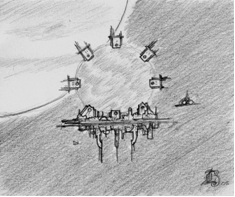
\includegraphics[width=120pt]{image/portail.png}}

Le second espace est une dimension parallèle à la nôtre. Une dimension où les lois de la physique, de l'espace, et du temps sont différentes. Il ressemble à un gigantesque océan secoué pas des courants puissants, imprévisibles, changeants. Un océan plongé dans une tempête permanente. Un océan aux milles couleurs.

Dans le second espace, il n'y a pas de planète. Des astres de notre monde, seuls les plus puissants tels que les étoiles ou les trous noirs ont une existence de l'autre coté. Il obeït à ses propres lois. L'équivalent de nos planètes dans cette dimension sont des zones de calme, des zones où les courants s'annulent, créant de petites poches de tranquillité. Ces zones sont remplies de créatures cherchant quelques minutes de repos.

Car le second espace est peuplé de créatures étranges, flottant au milieu de ce déchaînement d'énergie, évoluant dans ce milieu qui leur est naturel. La plupart de ces créatures sont innoffensives, mais les légendes parlent de monstres gigantesques capables de déchiqueter des vaisseaux entiers. D'autres racontent que les créatures chuchottent aux oreilles des voyageurs imprudents et les entraînent inexorablement vers la folie.

\subsection{Les Tellorias}

Au milieu du déchaînement d'énergie imprévisible qu'est le second espace, nous pouvons trouver un phénomène particulièrement intéressant : les Tellorias. Les Tellorias ressemblent à de puissants courants marins, des courants réguliers qui s'écoulent toujours dans la même direction, en suivant toujours le même itinéraire. 


Second point intéressant, les Tellorias sont doubles. A chaque Telloria correspond en réalité deux courants qui vont dans des sens opposés. Cerise sur le gâteau, les Tellorias semblent tenir éloignés les monstres les plus dangereux du second espace. Le système de portail créé par les Ergios tire justement profit des Tellorias.

\subsection{Naviguer dans le second espace}

Contre tout attente, la navigation dans le second espace a remis au gout du jour une vieille technologie de propulsion : la voile solaire. Le principe de la voile solaire est d'intercepter les flux de particules balayant constamment l'espace pour entraîner le vaisseau et accélérer petit à petit. Le second espace est justement un monde secoué en permanence par des vagues d'énergie !

La navigation dans le second espace se fait donc en déployant de grandes toiles énergetiques autour du vaisseau et en se laissant porter par les courants. Simple non ? En réalité, tout dépend de l'endroit dans lequel le vaisseau se trouve dans le second espace. En effet, un vaisseau rentrant dans une Telloria déploiera ses voiles et se laissera entraîner par le courant. C'est d'ailleurs ce que font la plupart des vaisseaux qui voyagent entre les systèmes.

Par contre, pour un vaisseau navigant en dehors des vagues Tellorias, l'affaire n'est pas aussi facile. Dans le second espace, pas de barre pour tenir le cap, seul un positionnement judicieux des voiles permet de se diriger dans la bonne direction. Les courants du second espace étant particulièrement imprévisibles, le pilote sera obligé de réajuster sans cesse les voiles.

De plus, il est extrêmement difficile pour un vaisseau de pénétrer dans une Telloria : les courants autour de la Telloria sont particulièrement forts et ont tendance à pousser les bâtiments loin de la vague.

\subsection{Pénétrer dans le second espace}

Aujourd'hui, les peuples des mondes connus connaissent trois technologies pour pénétrer dans le second espace : les portails, le moteur Solar, et le moteur Windsen.

L'utilisation d'un portail est la solution la plus répandue dans les voyages spatiales. Sur chaque système des mondes connus, les Ergios ont mis en place l'un de ces portails. Ceux-ci génèrent en continu une sorte de trou de ver. Chaque vaisseau qui le traverse se retrouve propulsé instantanément dans le second espace, au sein d'une Telloria. Cette technologie n'a qu'un seul souci : nous ne savons pas la recréer. Ce sont les Ergios qui ont bâti chaque portail et aujourd'hui nos scientifiques les plus pointus savent tous juste les maintenir en marche. Bien sûr, en démontant un générateur de portail nos scientifiques pourraient sûrement en apprendre plus, mais aucun système solaire n'est prêt à courir le risque d'être coupé du reste de la Fédération.

Le moteur Solar est une technologie assez récente, première avancée obtenue grâce à l'étude d'épaves Eskador. Le moteur Solar crée une perturbation qui, misd en présence d'une forte activité solaire, génère un trou de ver qui propulse le vaisseau dans le second espace. Il est toutefois nécessaire de s'approcher bien près du soleil tout en ayant une très grande vitesse pour que le moteur fonctionne. En cas de dysfonctionnement, c'est la mort assurée.

Le moteur Windsen en est encore au stade de prototype. Ce moteur est en réalité un générateur de trou de ver capable de transporter le vaisseau dans le second espace en parfaite autonomie. Le Bureau Corporatiste, à l'origine de cette technologie, place de grands espoirs dans son développement. Le défaut actuel du moteur Windsen est qu'il demande extrêmement d'énergie : un vaisseau utilisant ce moteur finirait son voyage quasiment à court de carburant...


Dans les trois solutions ci-dessus, seuls les portails permettent d'utiliser une Telloria. Les deux autres moteurs propulsent les vaisseaux en plein milieu de la tourmente. Seul un bon pilote saura mener son vaisseau à bon port.

\end{multicols}

\chapter{Combattre dans les mondes Fédéraux}

\begin{multicols}{2}

\section{La guerre spatiale}

\parpic[r]{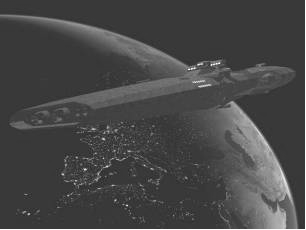
\includegraphics[width=120pt]{image/vaisseau1.png}}Dans la fédération, la guerre spatiale est une réalité presque devenue courante. Mais il faut bien comprend que la guerre spatiale est avant tout une guerre d’usure et de ressources : il est rare que deux flottes s’affrontent jusqu’à destruction totale.

En réalité, les vaisseaux spatiaux sont extrêmement complexes et si couteux à produire que les différentes forces rechignent à les sacrifier sans raison et tendent à limiter aux maximum les pertes.

La plupart des opérations militaires sont donc des opérations visant à limiter le commerce et l’approvisionnement d’un secteur. La technique privilégiée est alors l’abordage qui permet de récupérer les cargaisons plutôt que de les gâcher dans l’espace. 

Même en cas de combat entre deux flottes, les échanges de laser restent souvent un moyen d’affaiblir sans détruire le vaisseau adverse afin de pouvoir, par la suite, essayer de s’en saisir via un assaut. Le vaisseau ainsi capturé peut être réparé et récupéré dans les forces du vainqueur. 

Bien sûr, il y a des exceptions. Par exemple, les affrontements entre les flottes Teldrims et Humaines sont en général particulièrement violents.


\end{multicols}

\note{Les Abordages}{
Vous vous demandez peut-être pourquoi insister sur ce point et sur l’utilisation de la technique d’Abordage Spatial ? La raison est assez simple : l’abordage est une façon pratique de faire participer un maximum de personnages.

Lors d’un combat purement spatial, le nombre d’acteurs va être limité (un pilote et un artilleur, de temps en temps un mécano, un capitaine, et un co-pilote). Certains personnages risquent alors de s’ennuyer ferme. 

Rajouter un abordage en bonne et du forme, avec l’avancée ennemie à gérer, certaines zones dépressurisées, …, tout de suite, le nombre d’acteurs est démultiplié (et rien n’empêche de jouer sur les deux plans en même temps !).

Lors des abordages, surtout n’oubliez pas : un vaisseau spatial, c’est un peu comme un sous-marin : des couloirs étroits, des portes basses, des zones pressurisées qui s’isolent au moindre problème, des sas de sécurité, …}

\begin{multicols}{2}

\subsection{Combattre dans le second espace}

Est-il possible de combattre dans le second espace ? Dans la théorie, oui, rien ne l'empêche. Dans la pratique, les choses ne sont pas aussi simples.

Premièrement, la nature même de cette dimension rend les armes énergétiques complètements caduques. Or, la grande majorité des systèmes d'armement des vaisseaux récents sont constitués d'armes énergetiques. En réalité ces armes ne sont pas inutilisables, toutefois leur portée est réduite jusqu'à devenir insignifiante : il faut être à bout portant pour les utiliser.

Les armes à projectiles conservent, quand à elles, leur efficacité. Toutefois les courants d'énergie du second espace les influencent également et les fait dériver souvent loin de leurs cibles. Il faut un très bon artilleur et beaucoup de chance pour arriver à prévoir la dérive du projectile et à toucher son adversaire. 

Actuellement le combat en second espace est donc un affrontement à bout portant. Toutefois la plupart des gouvernements recherchent activement de nouveaux systèmes d'armement qui seraient adaptés à ce type de combat.

\end{multicols}
